 \subsection{Universidad de Mosku - Rusia}
Presentamos en la siguiente tabla los resultados obtenidos del último monitoreo.

\bigskip

\begin{tabular}{| l | c | c | c | c |}
 \hline 
Hop & IP &  RTT promedio (s)  & deltaRTT promedio & Ubicación\\
\hline 
1  &  192.168.0.1  &  0.003286 &  0.003286 & Argentina\\
\hline 
2  &  200.89.164.165  &  0.018267 &  0.014980 & Argentina\\
\hline 
3  &  200.89.165.130  &  0.018018 &  0 & Argentina\\
\hline 
4  &  200.89.165.222  &  0.023129 &  0.005110 & Argentina\\
\hline 
5  &  206.165.31.213  &  0.0159362 &  0 & United States\\ 
\hline 
6  &  67.17.75.66  &  0.153266 &  0.137330 &  United States\\
\hline 
7  &  4.68.111.121  &  0.144784 &  0 & United States\\ 
\hline 
8  &  4.69.158.253  &  0.267091    &  0.122307 &  United States\\
\hline 
9  &  4.69.158.253  &  0.266443    &  0 & United States\\
\hline 
10  &  213.242.110.198  &  0.313186    &  0.046742 & United Kingdom\\
\hline 
11  &  194.85.40.229  &  0.313147    &  0 & Russian Federation\\
\hline 
12  &  194.190.254.118  &  0.295875    &  0 & Russian Federation\\
\hline 
13  &  93.180.0.172  &  0.310500   &  0.014625 & Moscow City Russian Federation\\
\hline 
14  &  188.44.33.30  &  0.293746    &  0 & Moscow City\\
\hline 
15  &  188.44.50.103  &  0.286035   &  0 & Moscow City\\
\hline 
\end{tabular}

\bigskip
Con estos datos hemos obtenido que los $\Delta$ $RTT$ siguen una distribución normal con una probabilidad del 99,5$\%$ ($\alpha$ $=$ 0,005).
Se ha realizado el test de $Grubbs$ y nos ha devuelto que los $outliers$ se encuentran en los saltos 6 y 8.\\

A continuación mostramos que ocurre con los $RTT$ promedio de cada salto y con los $zScore$ promedio de cada salto:

\begin{figure}[H]
\centering
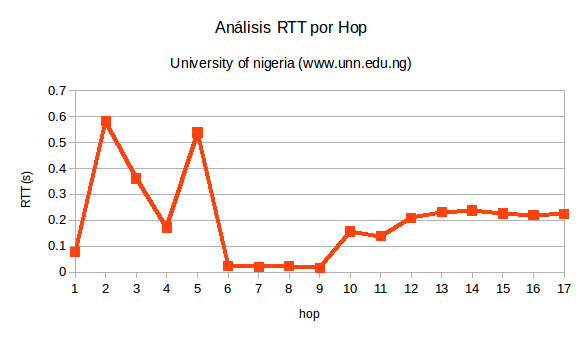
\includegraphics[width=1\textwidth]{graficos/zScore_rus.png}
\caption{zScore promedio por hop - Universidad de Mosku}
\label{Rus_zs}
\end{figure}

\begin{figure}[H]
\centering
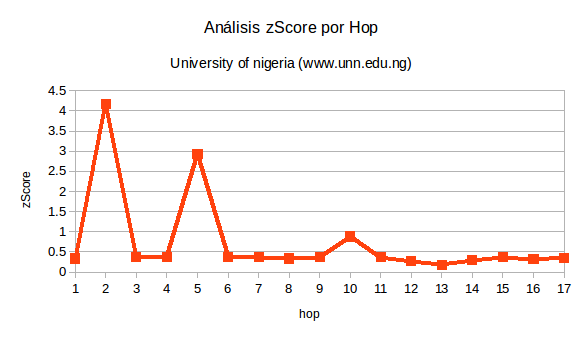
\includegraphics[width=1\textwidth]{graficos/RTT_rus.png}
\caption{RTT promedio por hop - Universidad de Mosku}
\label{Rus_rtt}
\end{figure}

De manera preliminar puede verse que la diferencia temporal entre los diferentes saltos permanece en el orden de los $10^-3$ segundos, 
habiendo tan solo dos casos en que esto no sucede. Primero en el salto 6 y luego en el salto 8 que se encuentran en el orden de los $10^-1$ 
segundos. Cómo en el caso de la universidad anterior corresponden a los saltos detectados como $outliers$.\\

Al calcular los $zScore$ apreciamos cuán alejados están los valores de la media.
Aquí también puede verse que los saltos 6 y 8 son los mas patológicos y por lo tanto, los mejores candidatos a ser enlaces submarinos.\\

Aún asi nos resulta extraño ver que tanto en el salto 6 como en el 8 las $IPs$ dicen estar asignadas a hosts de Estados Unidos. 
Suponemos que podría deberse a que aunque las $IPs$ esten asignadas a host de Estados Unidos, el lugar físico donde se encuentren sea otro.
Utilizando la herramienta http://www.infobyip.com/ pudimos observar algunos de los nombres de los hosts por los cuales hicimos el $traceroute$.

De esta herramienta conseguimos la siguiente información:\\

\bigskip
\begin{tabular}{| l | c | c |}
\hline 
hop & IP & Host name\\
\hline 
5  &  206.165.31.213  &  xe-8-3-0.ar3.eze1.gblx.net\\
\hline 
6  &  67.17.75.66  &   po3-20G.ar3.MIA2.gblx.net\\
\hline 
7  &  4.68.111.121  & ae5.edge2.miami2.level3.net\\
\hline 
8  &  4.69.158.253  & ae-114-3504.bar1.Stockholm1.Level3.net\\
\hline 
\end{tabular}
\bigskip

Tomando como hipótesis que los nombres de los hosts se corresponden con su ubicación geográfica, entonces nuestros resultados sobre 
cuales son los enlaces submarinos parecerían estar en lo correcto. Esto se debe a que del salto 5 al salto 6 el paquete habría viajado desde Argentina 
hacia Miami. Y del salto 7 al salto 8 el paquete parecería haber viajado de Miami hacia Estocolmo.

A continuación hemos trazado en un mapa la ruta de nuestro host hasta el host destino ubicado en Rusia tomando como cierta esta última información:
\begin{figure}[H]
\centering
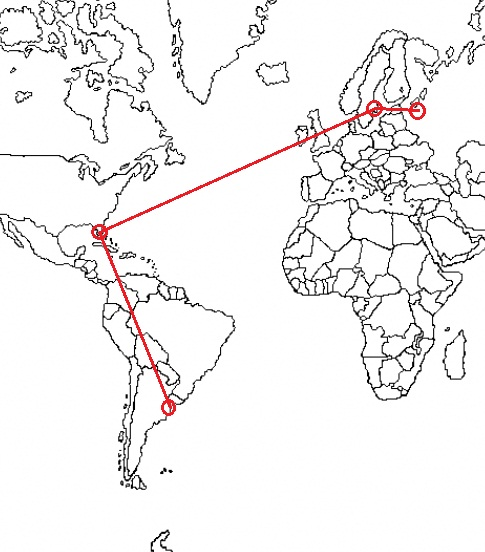
\includegraphics[width=0.8\textwidth]{graficos/mapa_rusia.jpg}
\caption{Ruta en Internet - Universidad de Mosku}
\label{rusia_zs}
\end{figure}